\chapter{Results}\label{cha:results}

This section will present and discuss the results from our experiments.
The modified SSD model presented in Section~\ref{sec:method-arch} is trained according to the training procedure given in Section~\ref{sec:method-exp-setup}.
Section~\ref{sec:results-baseline} presents the performance of the baseline model. 
The results from experiments pertaining to RQ1 and RQ2 are presented in Section~\ref{sec:results-simplification} and Section~\ref{sec:results-sharpness} respectively.
Unless specified otherwise, all performance metrics given in this section are measured on the test split of the dataset.

\section{Baseline model}\label{sec:results-baseline}
\begin{figure}[htb]
    \centering
    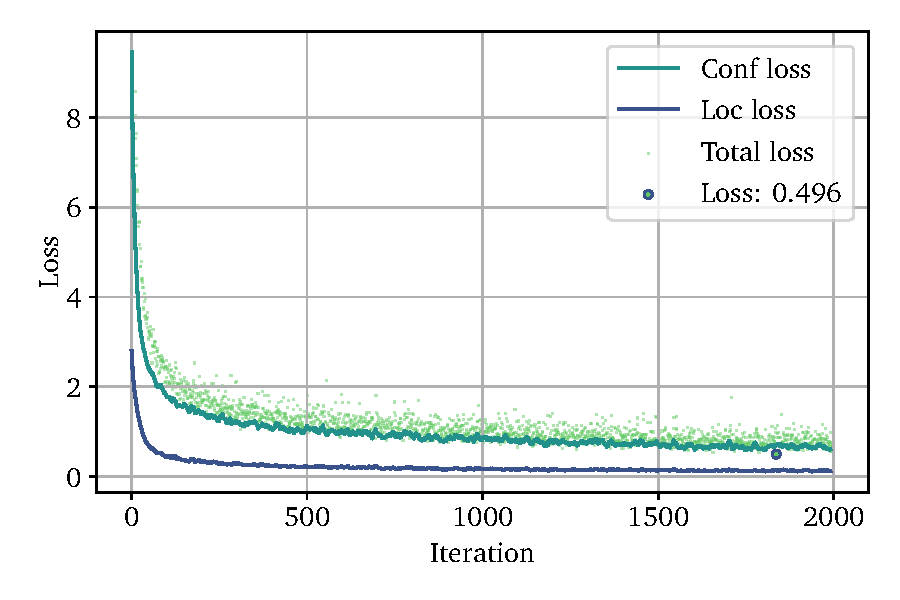
\includegraphics[width=0.7\textwidth]{figs/method/baseline/loss2.pdf}
    \caption[Baseline training procedure]{%
Training procedure for the baseline model over 2000 iterations.
The iterations are given on the horizontal axis are represent one forward-backpropagation run with one mini-batch, while the mini-batch averaged loss is given in the vertical axis.
The raw total loss values are shown with semi-transparent green points.
The solid lines show the moving means for the two individual loss components.
The green line shows the confidence loss component, while the blue line shows the localization loss component.
The mini-batch with the lowest total loss is annotated with a green circle and occurs after the 1600th iteration with a loss of 0.514.
    }\label{fig:method-baseline-loss}
  \end{figure}

We start by presenting the results from training the model in its baseline configuration. The training procedure is given in Figure~\ref{fig:method-baseline-loss}. The scattered loss is characteristic for mini-batch training. We can also see that the confidence loss accounts for most of the total loss throughout the training process. The components of the loss function (Equation~\ref{eq:loss}) are independent, meaning that their ratio does not indicate a difference in performance in the two different tasks. We do however observe that the model performs better at localization than classification.

\begin{figure}[htb]
    \centering
    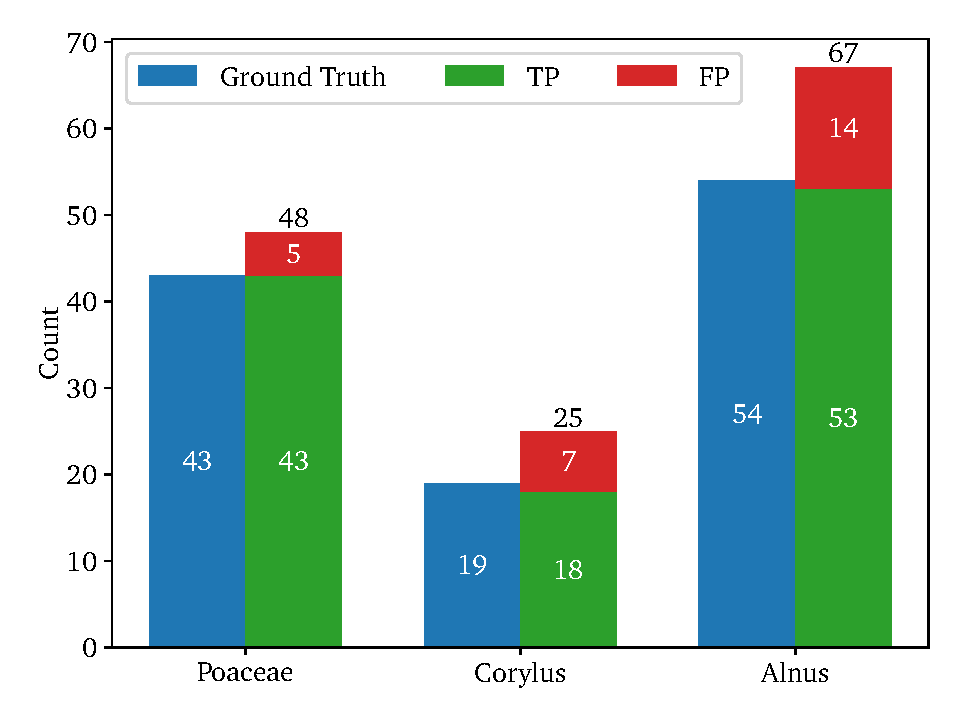
\includegraphics[width=0.7\textwidth]{figs/method/baseline/detections_test.pdf}
    \caption[Detections by type by class for the baseline on the test split] and an \(F_1\) score of 87.8\%.
Every ground truth is correctly localized (i.e.~it is identified by at least one bounding box of arbitrary class with an IoU above 0.5), meaning misclassification is the only source of error.
Figure~\ref{fig:method-baseline-detections} gives a breakdown of all the detections made



\section{Model simplification}\label{sec:results-simplification}

\section{Sharpness}\label{sec:results-sharpness}